\documentclass[]{scrartcl}
\usepackage{Preamble}
\usepackage{amsmath}

\renewcommand{\exercise}{Exercise 5}
\renewcommand{\duedate}{2020-07-06, 18:00}

\begin{document}
    \section{Simulations}
    \subsection{4x4 Crossbar}
    \begin{verbatim}
        Bestimmen und begründen Sie wie die Werte zustande kommen
    \end{verbatim}

    \begin{equation}
        Avg = \sum_{n=0}^N \frac{\binom{N}{n}\left( N-n+1 \right)! \cdot C_n }{\sum_{k=0}^N \binom{N}{k}\left( N-k+1 \right)!}
    \end{equation}

    \subsubsection{avg Input Queue Length}
        \begin{figure}[ht]
            \centering
            \includegraphics[width=\columnwidth, page=2]{../../python/results/preopt-General-0}
            \caption{Pre Optimization}%
            \label{fig:}
        \end{figure}

        \begin{itemize}
            \item Generated Packets
                \begin{itemize}
                    \item size: $ s = \SI{512}{b}$
                    \item send interval: $ t = \SI{512}{ns}$
                \end{itemize}
            \item Connection to XBar
                \begin{itemize}
                    \item data rate: $\SI{1}{Gbps}$
                \end{itemize}
        \end{itemize}

        \begin{align}
            r_\text{gen} &= \frac{\SI{512}{b}}{\SI{512}{ns}} = \SI{1}{Gbps}\\
            C_n &= \SI{250}{Mbps}\cdot n\\
            r_\text{q fill,eff} &= \sum_{n=1}^4 \frac{\binom{4}{n}\left( 5-n \right)! \cdot C_n }{141}\\
                                &= \SI{347.5}{Mbps}\\
            \Rightarrow l_\text{q, avg} &= \frac{t_\text{sim}\cdot r_\text{q fill, eff}}{2\cdot s} = 3394
        \end{align}

    \subsubsection{avg End-to-End Latency}
    \begin{figure}[ht]
        \centering
        \includegraphics[width=\columnwidth, page=8]{../../python/results/preopt-General-0}
        \caption{Pre Optimization e2e latency}%
        \label{fig:preopt-2e2}
    \end{figure}
        \begin{itemize}
            \item (no delays inside buffers, because the generated data rate, even for all 4 apps, is lower than a single data rate channels maximum throughput)
            \item minimum
                \begin{itemize}
                    \item App $\rightarrow$ C $\rightarrow$ Inport
                        $\rightarrow$ C $\rightarrow$ Outport $\rightarrow$ C $\rightarrow$ App
                    \item delay for packet: $t_{delay}=512ns$ (per \verb|DatarateChannel| C)
                        \begin{equation}
                            \Rightarrow t_{e2e,min} = \SI{1.536}{\mu s}
                        \end{equation}
                \end{itemize}
            \item maximum

                at end of simulation, inport buffer full, all in to one out

                \begin{align}
                    l_{inport q, max} &= 7031\\
                    r_{dequeue, min} &= \SI{250}{Mbps}\\
                    t_\text{in queue, max} &= \frac{t_{q,inport}\cdot s}{r_{dequeue}} = \SI{3.599}{ms}\\
                \end{align}

            \item on avg
                \begin{align}
                    t_\text{e2e, avg} &= t_\text{in queue, max} / 2 = \SI{1.8}{ms}
                \end{align}

        \end{itemize}

    \subsubsection{avg Arbiter Request Queue Length}
    \begin{figure}[ht]
        \centering
        \includegraphics[width=\columnwidth, page=4]{../../python/results/preopt-General-0}
        \caption{Pre Optimization Queue Length}%
        \label{fig:postopt-General-0}
    \end{figure}
        \begin{itemize}
            \item cases
                \begin{align}
                    C_n &= n-1 \qquad 1\leq n\leq4=N
                \end{align}
            \item on avg (analogously to $t_{e2e}$)
                \begin{equation}
                    \Rightarrow l_{arbq,avg} = \sum_{n=1}^4 \frac{\binom{4}{n}\left( 5-n \right)! \cdot C_n }{141} = 0.39
                \end{equation}
        \end{itemize}
    \subsubsection{avg Arbiter Request Queue Time}
        \begin{figure}[ht]
            \centering
            \includegraphics[width=\columnwidth, page=7]{../../python/results/preopt-General-0}
            \caption{Pre Optimization Arbiter Queue Times}%
            \label{fig:preopt-arbiter-qtime}
        \end{figure}
        \begin{itemize}
            \item cases
                \begin{align}
                    C_n &= \SI{512}{ns} * n
                \end{align}
            \item on avg
                \begin{align}
                    \Rightarrow t_{arbq,avg} &= \sum_{n=1}^4 \frac{\binom{4}{n}\left( 5-n \right)! \cdot C_n }{141}\\
                                             &=
                \end{align}
        \end{itemize}

    \subsubsection{avg Output Buffer Queue Length}
        \begin{figure}[ht]
            \centering
            \includegraphics[width=\columnwidth, page=6]{../../pthon/results/preopt-General-0}
            \caption{../../pthon/results/preopt-General-0}%
            \label{fig:../../pthon/results/preopt-General-0}
        \end{figure}
        \begin{itemize}
            \item Generated Packets
                \begin{itemize}
                    \item size: $ s = \SI{512}{b}$
                    \item send interval: $ t = \text{uniform}(\SI{1}{\mu s}, \SI{10}{\mu s}) = \SI{5.5}{\mu s}$
                \end{itemize}
            \item Connection to and in XBar
                \begin{itemize}
                    \item data rate: $\SI{1}{Gbps}$
                \end{itemize}
        \end{itemize}
        \begin{align}
            r_\text{generated} =& \frac{\SI{512}{b}}{\SI{5.5}{\mu s}} = \SI{93}{Mbps}\\
            \Rightarrow l_\text{q,avg} = 0
        \end{align}
    \begin{itemize}
        \item \verb|avg Throughput|

            input and output buffers always empty
            \begin{align}
                r_{cross} &= 4*r_\text{gen}\\
                &= \SI{372}{Mbps}
            \end{align}
    \end{itemize}
    \subsection{Throughput vs. Ports}
    \begin{itemize}
        \item with our formula
            {0.6, 0.44, 0.347518, 0.286498, 0.243324, 0.211277, 0.186604, 0.167047, 0.151176, 0.138045,

    0.127005, 0.117594, 0.109478, 0.102407, 0.0961928, 0.0906881, 0.0857783, 0.0813722, 0.077396,

    0.0737899, 0.0705046, 0.067499, 0.0647391, 0.0621958, 0.0598446, 0.0576646, 0.0556378, 0.0537485,

    0.0519832, 0.0503302, 0.048779}
    \end{itemize}
    \subsection{Throughput vs. Injection Rate}
    \begin{itemize}
        \item not in saturation until delay $\leq \SI{832}{ns}$
        \item saturation point $r_{sat} = \frac{\SI{512}{b}}{\SI{832}{ns}} = \SI{615}{Mbps}$
        \item The main reason will be the arbiter. It can only process packets at about \SI{600}{Mbps} on avg., therefore bottlenecking the rest of the system
    \end{itemize}
    \subsection{Throughput vs. Bandwidth}
    \begin{itemize}
        \item Network in saturation until bandwidth $> \SI{1600}{Mbps}$
        \item throughput at saturation point $r_{sat} = \SI{1}{Gbps}$
        \item If the Arbiter can only work at $\approx$ 62\% of the bandwidth, we reach this saturation point if 62\% of the bandwidth is \SI{1}{Gbps}, therefore the required bandwith is \SI{1613}{Gbps}
    \end{itemize}
\section{Optimizations}
\subsection{Problems}
In the previous exercise we determined the arbiter to be the limiting resource.
We determined head of line blocking to be a limiting factor for performance.
Since packets are sent to random nodes it is very likely for a packet having to
wait because the route is currently occupied even though other packets in queue
could be routed.
Therefore virtual queues were implemented.

\subsection{Solution}
We can measure the performance gain in correlation to the average inport buffer
length which is decreased by two orders of magnitude. Form around 3000 to around
15

\subsection{Problems In Real Hardware}
In a real hardware setting this would increase complexity.
Either distinct buffers have to be used or some sort of control logic that holds
pointers to the virtual queues. Spatial constraints have to be taken into account
as well as scalability. With more possible routing decisions the number of virtual
queues also rises.

\begin{figure}[ht]
    \centering
    \includegraphics[width=\columnwidth, page=2]{../simulations/results/General-0}
    \caption{sim}%
    \label{fig:optsim_inport_qlen}
\end{figure}
\begin{figure}[ht]
    \centering
    \includegraphics[width=\columnwidth, page=8]{../simulations/results/General-0}
    \caption{}%
    \label{fig:}
\end{figure}
\begin{figure}[ht]
    \centering
    \includegraphics[width=\columnwidth, page=4]{../simulations/results/General-0}
    \caption{}%
    \label{fig:}
\end{figure}
%\includegraphics[width=\columnwidth, page=5]{../simulations/results/General-0}

\end{document}
